% Chapter 4
\chapter{Transmission Expansion Planning by Quantum Annealing} % Main chapter title
\label{Chapter4} % For referencing the chapter elsewhere, use \ref{Chapter1} 
\section{Statement of the problem}
\textit{Transmission expansion planning} (TEP)\,\cite{Neumann2020TransmissionFlows} is a \textit{mixed integer linear programming} (MILP) problem that aims at finding the optimal way to expand the capacity of an energy system by reducing the cost function which is the sum of the investment cost of transmission lines and the operational cost of generators. It decides how many transmission lines to build and where to connect them in order to satisfy the energy demand on a distributed energy system with a high share of renewable energy sources. There are other components to build apart from transmission lines such as generators or storages, but considering them imply not only an increment in the number of variables of the problem but also an increment in the complexity to formulate it. The problem we are solving is not realistic at all, so we should consider it just as a starting point to get insight about the problem formulation and challenges.\\\\
We can control the number of variables of the problem according to
\begin{itemize}
    \item \textbf{Number of nodes:} Clustering techniques allow us to fix the number of nodes of the problem so that towns of a given network are grouped acting as a single big town.
    \item \textbf{Snapshots of time}: In expansion problems is common to consider hourly snapshots of time of one year, i.e., a total of 8760 snapshots but we can restrict the problem to a subset of snapshots without loss of generality.
    \item \textbf{Connectivity of transmission lines}: We can control the connectivity between nodes so that we do not allow a node the possibility of being fully connected with the rest of nodes. Furthermore, because of legal procedures to build new lines in areas where there were no transmission lines, TEP focus on building lines in existing connections without changing the topology of the network.
    \item \textbf{Adding targets}: In this chapter we tackle a single target, i.e., the cost function -- investment and operational cost -- but there are other targets such as the increment of renewable energy sources in a given region or the reduction of the carbon footprint.
\end{itemize}
The TEP scales badly using classical algorithms\,\cite{Oertel2014ComplexityEvaluation} and, at the same time, energy system models are getting larger and more complex due to the integration of decentralized weather-dependent renewable energy sources, intermittent loads, sector coupling and the increase of storage components. Currently, the problem is often linearized or the scope and granularity of the model are reduced using clustering algorithms. For this reason, any computational time reduction will have substantial implications in closing the granularity gap between what the current models can solve and the desired resolution needed by energy system operators. Because of the maturity of quantum computers large TEP problems cannot be solved fully by a quantum annealer. For this reason, we require of hybrid methods\,\cite{Ding2019ImplementationDesign,Zhao2021HybridProgrammingb} to decompose large problems into a master problem which can be solved by a quantum annealer and a sub-problem for which cutting-edge classical algorithms are going to be applied.\\\\
There are two ways of formulating the transmission expansion problem. In one hand, the brownfield model considers the power flow of existing in a network $f_{kl}^{(0)}$ among with the power flow of a set of candidate lines $f_{kl}^{(1)}$. On the other hand, the greenfield model considers a empty network and a set of candidate lines $f_{kl}^{1}$.
\begin{figure}[H]
  \begin{center}
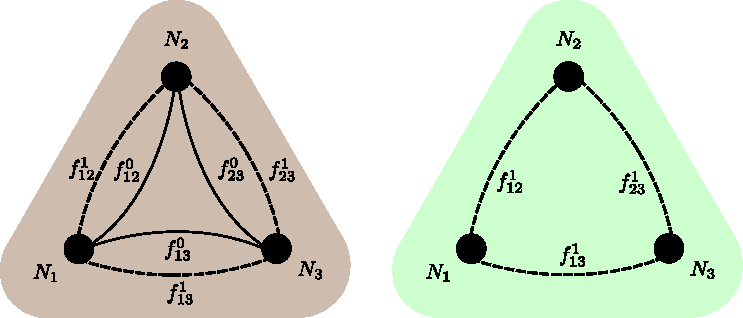
\includegraphics[width=0.9\textwidth]{Figures/3NodeBrownGreen.pdf}
  \end{center}
  \caption{Three node example. \textbf{Right:} Network considering current transmission lines and candidate lines, brownfield model. \textbf{Left:} Network considering just candidate lines, greenfield model.}
  \label{fig: ThreeNode}
\end{figure}
For simplicity, we are gonna consider the greenfield approach so we do not have to take into account the constants associated with the existing lines. We can map two indexes $ij$ to a single index $k$ by using a bijective function for a given number of nodes $N$, see Ref.\,\cite{Jain2021SolvingComputer},
\begin{equation}
k(i,j,N) = \begin{cases}
    iN - i\left(i+1\right)/2 + j - (i+1), & i<j\\
    \text{None},& i=j \\
    k(j,i,N), & i>j
\end{cases}
    \label{eq: TwoIndexesmap}
\end{equation}
Luckily, the \textit{dimod} python package from D-Wave allow us to name the variables so that we do not need to use the previous function to reformulate the problem. We formulate the TEP problem according to the work of Dilwali \textit{et al.}\,\cite{Dilwali2016},
\begin{mini!}[1]
	{\mathbf{l},\mathbf{g}}{\underbrace{\sum_{kl\in C}c_{kl}x_{kl}}_{\text{Investment cost}} + \underbrace{\sum_{h\in H}^{H}\sum_{k}c_{k}^{(\text{oc})}g_{k}(h)}_{\text{Operational cost}} + \underbrace{\sum_{k}r_{k}c_{k}}_{\text{Load shedding cost}}}{\label{eq: objective}}{}{}
	\addConstraint{d_{k}(h)-\sum_{l\in E_{k}}f_{kl}^{0}(h) + \sum_{l\in C_{k}}f_{kl}^{1}(h) + g_{k}(h)}{=0,}{\forall k\in N ,h\in H}
    \addConstraint{\abs{f_{kl}^{0}} - \bar{f_{kl}^{0}}}{\leq 0,\,}{\forall\, kl \in E }
     \addConstraint{\abs{f_{kl}^{1}} - \bar{f_{kl}^{1}}}{\leq 0,\,}{\forall\, kl \in C }
     \addConstraint{g_{k}(h)-\bar{g}_{k}}{\leq 0,\,}{\forall\, k\in N,h\in H }
    \addConstraint{r_{k} - d_{k}}{\leq 0,\,}{\forall\, k \in N }
    \addConstraint{x_{kl}}{\in \{0,1\},\,}{\forall\, kl \in C.}
\end{mini!}
Notice that we include the operational cost which is usually not included in the literature (\textbf{INCLUIR LOS PAPERS RELEVANTES}). The reason of not including the operational cost is that they are considering a single snapshot so that the dominant term is the investment cost and the operational cost can removed from the objective function. However, if one wants to consider large snapshots, then the operational cost is the dominant term. Furthermore, if we just minimize the investment cost, then we can build lines that connect the most expensive generators. Moreover, if we consider a large set of snapshots $h$, then the operational cost is the dominant term. Analogously, for a short set of snapshots the investment cost is the dominant term of the total cost function. In summary, extremal solutions lead to a high value of cost function in one of these ways
\begin{itemize}
    \item \textbf{Underinvestment} leads to a high value of the total cost function because the system is not able to fulfill the demand $d(h)$.
    \item \textbf{Overinvestment} leads to a high value of the total cost function despite it fulfill the demand. Intuitively, we are creating more elements $\{x_{kl}\}$ than we need. Usually there is an upper bound due to the capital budget.
\end{itemize}
The TEP combinatorial optimization problem is a trade-off between operational cost and investment cost where the optimal solution minimize the investment cost and operational cost fulfilling at the same time the constraints of the problem.\\\\
We can write the problem as a Hamiltonian by including the penalty terms,
\begin{equation}
    \mathcal{H} = \sum_{k=1}^{L}c_{k}^{(\text{iv})}x_{kl} + \sum_{t=1}^{T}\sum_{j=1}^{G}c_{j}^{(\text{oc})}g_{j}^{(\text{fixed})}(t) + P\left[\sum_{i}\sum_{t}\left(D_{i}(t) - \sum_{j=1}^{G}g_{j}^{(\text{fixed})}(t)l_{k(i,j,N)}\right)^{2}\right]
\end{equation}
The meaning of the variables is explained in the following table
\begin{table}[H]
\centering
\begin{tabular}{|c||c|c|} 
 \hline	
 \textbf{Symbol} & \textbf{Description} & \textbf{Type} \\
 \hline	
 $N$ & Total number of nodes & Integer\\
  \hline	
  $H$ & Set of snapshots & Integer\\
  \hline
 $C$ & Set of candidate transmission lines & Integer\\
    \hline	
 $C_{k}$ & Set of candidate transmission lines from all nodes to node $k$ & Integer\\
  \hline	
 $E$ & Set of existing transmission lines & Integer\\
   \hline	
 $E_{k}$ & Set of existing transmission lines from all nodes to node $k$ & Integer\\
  \hline	
 $G$ & Total number of generators & Integer\\
  \hline	
 $T$ & Total number of snapshots & Integer\\
  \hline	
 $x_{kl}$ & Transmission line from node $k$ to node $l$ & Binary\\
  \hline
  $c_{kl}$ & Investment cost of transmission line from node $k$ to node $l$ & Integer\\
  \hline
  $r_{k}$ & Shedding load at bus $k$ & Integer\\
  \hline	
 $d_{k}(t)$ & Demand of node $i$ at snapshot $t$ & Integer\\
  \hline	
 $g_{k}(t)$ & Current generation at node $k$ at snapshot $t$ & Integer\\
  \hline	
 $\bar{g}_{k}$ & Maximum generation at bus $k$ & Integer\\
  \hline	
 $c_{k}^{(\text{iv})}$ & Investment cost of line $k$ & Real\\
  \hline	
  $c_{j}^{(\text{oc})}$ & Annualised operational cost per MWh of generator $g_{j}$ & Real\\
  \hline
  $c_{k}$ & Cost of shedding load at bus $k$ & Real\\
  \hline
\end{tabular}
\caption{Description of variables involved in TEP problems}
\label{table:TEPNomenclature}
\end{table}
The investment cost $c_{k}^{(\text{iv})}$ is the cost of building the transmission line $x_{kl}$ and it is a constant -- we are not considering time-dependent costs --, analogously, the operational cost $c_{j}^{(\text{oc})}$ represents the annualised cost per [MWh] of the produced energy $g_{j}(t)$ at time $t$. For simplicity, we set the operational cost to each carrier -- wind turbine, solar or run of river among others -- to a fixed value -- mean cost of that carrier -- so that we do not have to consider the variation of the cost as function of the node or the time.\\\\
Notice, that the total cost depends on the investment cost and the operational cost. As stated before the number of possible configurations of our problem scale badly. For this reason, knowing if we are considering a large set of snapshots -- large investment planning - or just a tiny subset of snapshots gives us clues about what region of the configuration space we should explore. There are two regions to be considered,
\begin{itemize}
    \item \textbf{Large expansion planning:} Consider we are given a 10 year expansion planning problem, then if we produce the energy with the  cheapest carriers -- e.g. wind turbines -- we will reduce the operational cost drastically as compared with producing the energy with other carriers. Maybe the fact of producing the energy with the cheapest carriers implies we build the more expensive transmission lines, hence increasing the investment cost.
    \item \textbf{Short expansion planning:} Consider a single-snapshot, then it is obvious that the minimum total cost function imply a minimum in the investment cost regardeless of the operational cost, since the operational cost are lower as compared with the investment cost and only have one snapshot to act.
\end{itemize}
This trade-off between investment cost and operational cost is what determine the minimum value of the total cost function.\\\\
To summarise, we receive as input a given energy demand for a set of nodes $i$ for a set of snapshots $t$, then we optimise the network so that we build the minimum amount of transmission lines -- minimizing in that way the investment cost -- so that the energy demand is satisfied for each snapshot. We are also taking into account the operational cost of each carrier so there is a trade-off between the investment cost of transmission lines and the operational cost of generators used to produce the energy to satisfy the demand.
%%%%%%%%%%
\section{Running QUBO problem on D-WAVE's annealer}

\subsection{Three-Node without discretization in transmission capacities}
In this example we solved the three-node network with three candidate lines where the transmission capacities are fixed, i.e., if a line transmit electricity it does it always with the same value. In this way we can simplify the problem by not using slack variables for discretizing the transmission capacities.\\\\
D-Wave\,\cite{D-WaveDocumentation} allows us to formulate the QUBO by hand and use the  solver .... or we can .... using CQM ....
\section{Benders Decomposition in TEP}
TIENE SENTIDO SI NO PODEMOS USAR UN QUANTUM ANNEALER? PODEMOS UTILIZAR EL MIN DE CALCULO MENSUAL

